\newcommand{\smathn}[1]{\scalebox{0.45}{$#1$}}

\begin{figure*}[t]
\centering

\begin{adjustbox}{max width=\textwidth}
\begin{tikzpicture}[
  ampersand replacement=\&,
  >=Latex,
  node distance=0.45cm and 0.55cm,
  pipelinearrow/.style={
    -{Latex[length=2.5mm,width=1.8mm]},
    line width=0.9pt,
    draw=black
  },
  newlabel/.style={
    font=\sffamily\bfseries\LARGE,
    text=red,
    anchor=south,
    inner sep=1pt
  },
  arxivlabel/.style={
    font=\tiny,
    text=red,
    anchor=south,
    inner sep=1pt
  },
  pipelinethinarrow/.style={
    -{Latex[length=2.1mm,width=1.5mm]},
    line width=0.7pt,
    draw=black
  },
  process/.style={
    draw=black!75,
    line width=0.7pt,
    rounded corners=1pt,
    fill=orange!7,
    inner sep=5pt,
    align=left
  },
  logo/.style={
    draw=black!70,
    rectangle,
    rounded corners=3pt,
    fill=blue!4,
    minimum width=0.5cm,
    minimum height=0.8cm,
    inner sep=2pt,
    align=center
  },
  imagebox/.style={
    draw=black!65,
    line width=0.5pt,
    fill=white,
    inner sep=1.5pt
  },
  tablebox/.style={
    draw=none,
    fill=white,
    inner sep=0pt,
    outer sep=0pt,
    minimum width=0pt,
    minimum height=0pt,
    align=center
},
  pairbox/.style={
    draw=black!75,
    line width=0.7pt,
    fill=white,
    inner sep=1.5pt,
    outer sep=0pt,
    align=center
},
  llm/.style={
    draw=black!75,
    line width=0.7pt,
    fill=orange!7,
    inner sep=5pt,
    align=left
},
  instruction/.style={
    draw=black!75,
    line width=0.7pt,
    fill=orange!4,
    inner sep=3pt,
    align=left
},
  imageencoder/.style={
    draw=black!80,
    line width=0.8pt,
    trapezium,
    trapezium left angle=70,
    trapezium right angle=70,
    shape border rotate=270,
    minimum width=1.1cm,
    minimum height=0.8cm,
    fill=blue!10,
    align=center
}
]

\node[logo] (arxiv) at (0,0) {%
    
\includegraphics[width=1.00cm]{structure/logos/arxiv-logo.png}
};

\node[logo, right=0.055cm of arxiv] (github) {%
    
\includegraphics[width=0.6cm]{structure/logos/github-mark.png}
};

\node[logo, right=0.055cm of github] (tex) {%
    
\includegraphics[width=1.00cm]{structure/logos/se-logo.png}
};

\node[
    process,
    below=0.45cm of github,
    text width=2.66cm,
    align=left
] (filter) {
    \small
    \textbf{Data Preprocessing}\\
    \vspace{0.2em}
    \scriptsize
    \textbullet\ TikZilla Filtering \\
    \textbullet\ Rendering \\
    \textbullet\ Grouping \\
    \vspace{-0.55em}
    \textbullet\ Pruning
};

\node[
    anchor=north east,
    inner sep=0pt
] at ($(filter.north east)+(0.0cm,-1.3cm)$) {%
    
\includegraphics[width=0.5cm]{structure/logos/filter.png}
};

\draw[pipelinethinarrow]
    (arxiv.south) -- ++(0,-0.20)
    -| ($(filter.north west)+(0.42cm,0)$);

\draw[pipelinethinarrow]
    (github.south) -- ($(filter.north)+(0,0)$);

\draw[pipelinethinarrow]
    (tex.south) -- ++(0,-0.20)
    -| ($(filter.north east)+(-0.42cm,0)$);

\node[imagebox, anchor=north west] (pathone)
    at (3.5,0.13) {%
        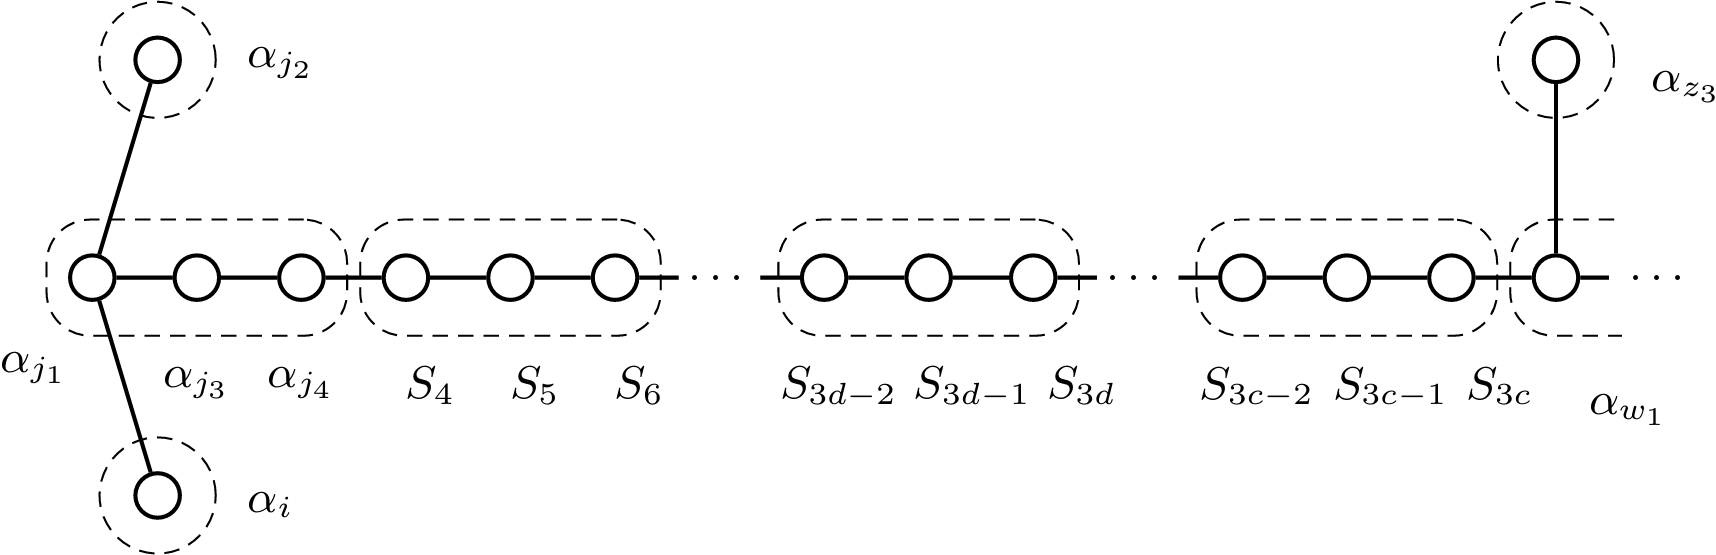
\includegraphics[
            width=1.5cm,
            height=0.5cm,
            keepaspectratio
        ]{structure/figures_dataset/structure_1.png}
    };

\node[imagebox, anchor=north west] (pathtwo)
    at (4.2,-0.5) {%
        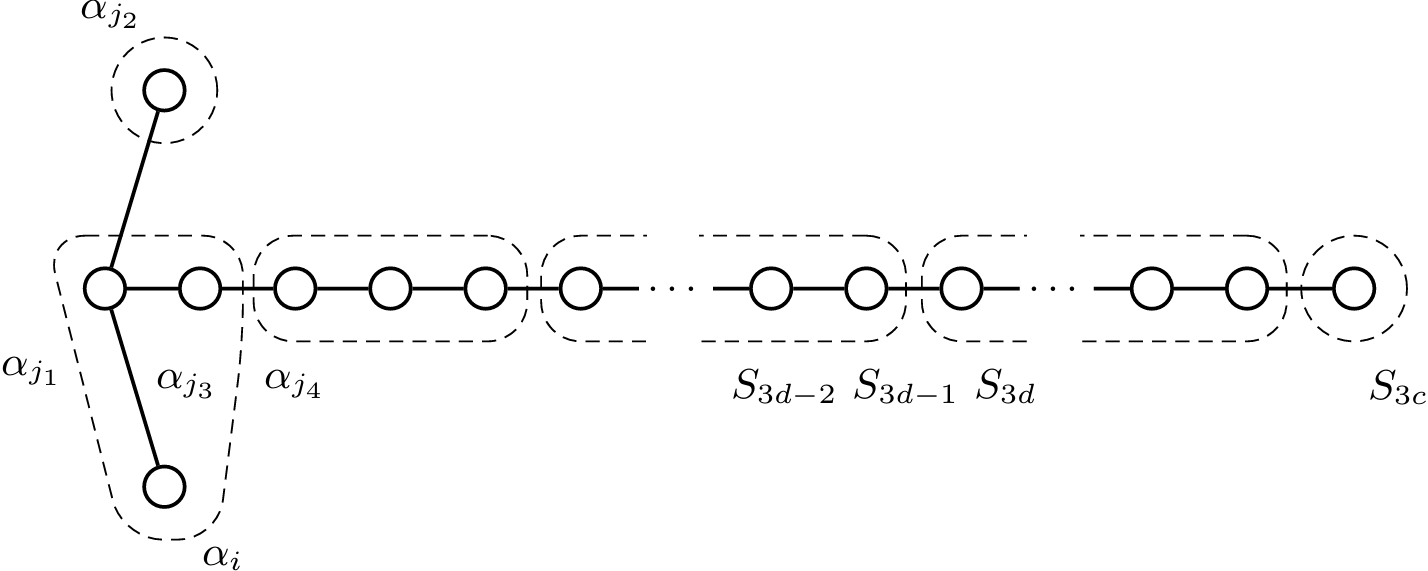
\includegraphics[
            width=1.5cm,
            height=0.5cm,
            keepaspectratio
        ]{structure/figures_dataset/structure_2.png}
    };

\node[imagebox, anchor=north west] (heatmap)
    at (4.2,-1.15) {%
        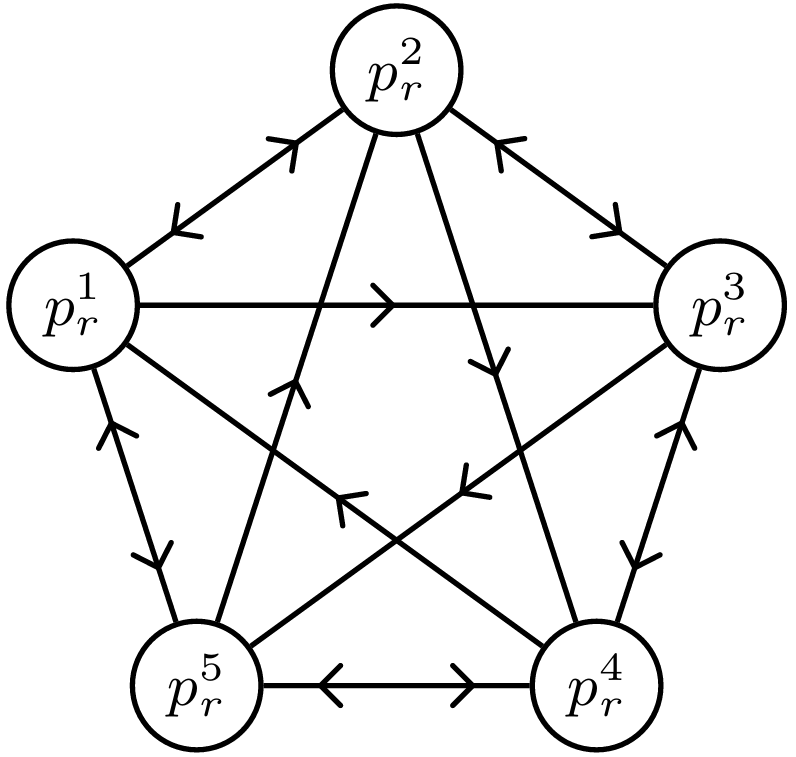
\includegraphics[
            width=0.95cm,
            height=0.95cm,
            keepaspectratio
        ]{structure/figures_dataset/penta_path.png}
    };

\node[imagebox, anchor=north west] (verticalchart)
    at (3.0,-0.5) {%
        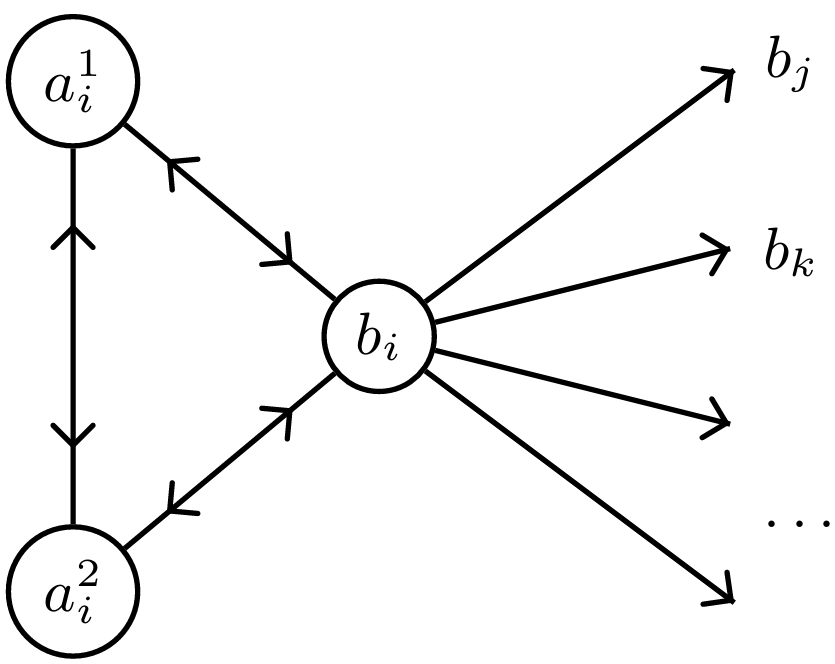
\includegraphics[
            width=1.05cm,
            height=1.05cm,
            keepaspectratio
        ]{structure/figures_dataset/path_node_edge.png}
    };

\node[newlabel] at (3.7,-2.0) {...};

\node[arxivlabel] at (4.3,-2.4) {arxiv/2107.04368};

\draw[pipelinethinarrow]
    (filter.east) to +($(0.33cm,0)$);

\draw[
  red,
  line width=1pt,
  dash pattern=on 5pt off 4pt
]
  (4.3,-1.10)
  ellipse [x radius=1.5cm,y radius=1.5cm];

\node[
    imageencoder,
    anchor=center
] (encoder) at (6.76,-0.2) {%
    \footnotesize IE
};

\node[
    tablebox,
    below=0.6cm of encoder
] (embmatrix) {%
{
\fontsize{3}{3.5}\selectfont
\setlength{\tabcolsep}{0.0pt}
\renewcommand{\arraystretch}{1.5}
\begin{tabular}{ccc}
\toprule
$\mathbf{e_1}$ & $\cdots$ & $\mathbf{e_N}$\\
\midrule
$-0.45$ & $\cdots$ & $0.52$\\
$0.03$ & $\cdots$ & $-0.01$\\
$0.27$ & $\cdots$ & $-0.79$\\[-2em]
$\vdots$ & $\ddots$ & $\vdots$\\
$0.82$ & $\cdots$ & $0.21$\\
\bottomrule
\end{tabular}
}
};

\draw[pipelinearrow]
    (encoder.south) -- ++(0.0,-0.6cm);

\draw[pipelinearrow]
    (5.5cm,-0.2cm) -- (encoder.west);

\node[
    tablebox,
    right=0.15cm of embmatrix,
    yshift=-0.1cm
] (simmatrix) {%
{
\fontsize{3}{3.5}\selectfont
\setlength{\tabcolsep}{0.7pt}
\renewcommand{\arraystretch}{1.15}
\begin{tabular}{c|cccc}
    & $\mathbf{i_1}$ & $\mathbf{i_2}$ & $\cdots$ & $\mathbf{i_N}$\\
\midrule
$\mathbf{i_1}$
    & $1.00$ & \textcolor{blue}{$0.98$} & $\cdots$ & \textcolor{red}{$0.92$}\\
$\mathbf{i_2}$
    & \textcolor{blue}{$0.98$} & $1.00$ & $\cdots$ & \textcolor{red}{$0.86$}\\[-2em]
$\vdots$
    & $\vdots$ & $\vdots$ & $\ddots$ & $\vdots$\\
$\mathbf{i_N}$
    & \textcolor{red}{$0.92$} & \textcolor{red}{$0.86$} & $\cdots$ & $1.00$\\
\end{tabular}
}
};

\draw[pipelinearrow]
    ($(embmatrix.east)+(-0.1,0)$)
    -- ++(0.4,0);

\node[
    pairbox,
    above=0.35cm of simmatrix
] (retainedpair) {%
    \begin{minipage}{1.9cm}
        \centering
        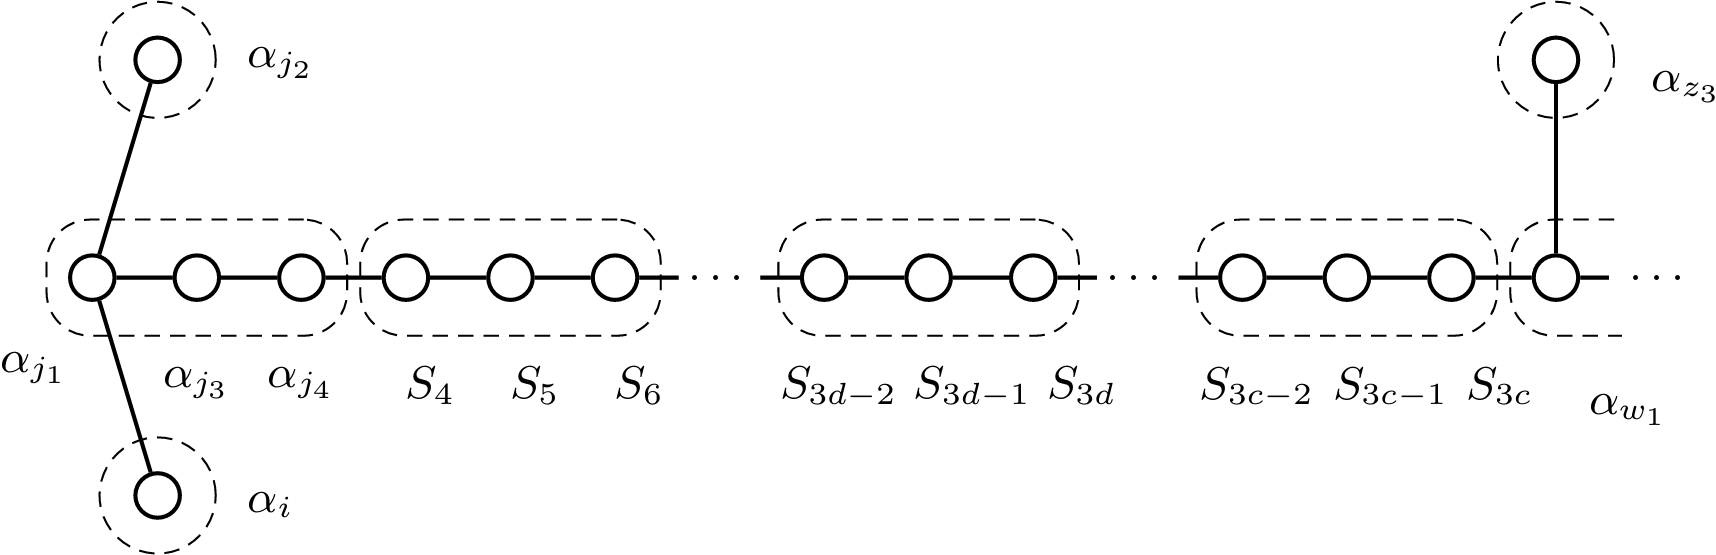
\includegraphics[
            width=2cm,
            height=0.75cm,
            keepaspectratio
        ]{structure/figures_dataset/structure_1.png}
        \\[-1.0em]
        \hspace*{0.6mm}\rule{1.85cm}{0.45pt}
        \\%[-0.15em]
        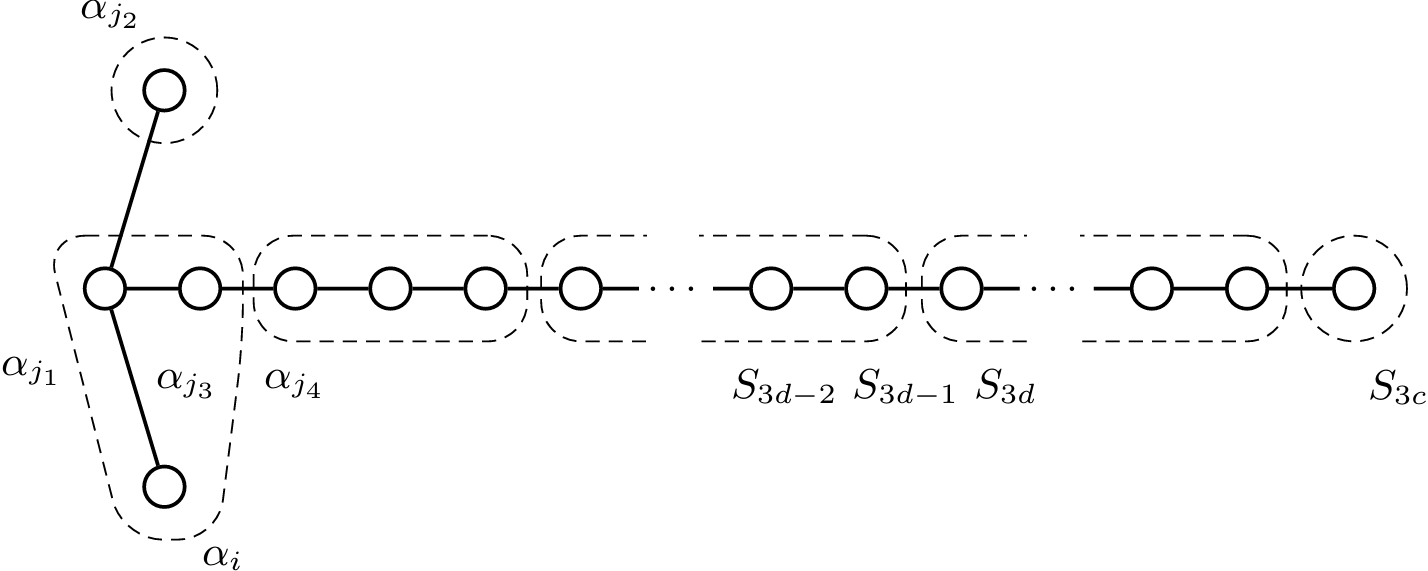
\includegraphics[
            width=2cm,
            height=0.75cm,
            keepaspectratio
        ]{structure/figures_dataset/structure_2.png}
    \end{minipage}
};

\draw[pipelinearrow]
    (simmatrix.north)
    -- (retainedpair.south);

\node[
    llm,
    right=0.35cm of retainedpair,
    yshift=0.11cm,
    minimum width=2cm,
    minimum height=0.7cm
] (vlmblock) {%
    \begin{minipage}{2.1cm}
    \small
        \textbf{VLM Editing}\\
        \tiny
        Analyze differences between Image X + TikZ X and Image Y + TikZ Y...
    \end{minipage}
};

\node[
    anchor=north east,
    inner sep=0pt
] at ($(vlmblock.north east)+(-0.02cm,-0.04cm)$) {%
    
\includegraphics[width=0.38cm]{structure/logos/ai-assistant.png}
};

\draw[pipelinearrow]
    (retainedpair.east)
    -- (vlmblock.west |- retainedpair.east);

\node[
    below=0.35cm of vlmblock,
    inner sep=0pt,
    outer sep=0pt,
    draw=none,
    fill=none,
    align=center
] (instructionblock) {%
    {
    \setlength{\tabcolsep}{0.08cm}
    \begin{tabular}{
        @{}
        p{1.25cm}
        @{\hspace{0.08cm}
        }
        p{1.25cm}
        @{}
    }
    \specialrule{0.55pt}{0pt}{-0.4em}
    \centering
    \fontsize{4.2}{4.5}\selectfont
    \textbf{Forward}\\[-0.5em]
    \rule{1.0cm}{0.4pt}\\[0.12em]

    \raggedright
    \fontsize{2.9}{3.2}\selectfont
    ``Delete the continuation to the right of the node labeled
    \smathn{S_{3c}}: remove the adjacent node labeled
    \smathn{\alpha_{w_1}}, the following horizontal ellipsis, the upper
    node labeled \smathn{\alpha_{z_3}}...''
    
    \vspace{0.2em}
    \textbullet\ Delete node labels\\
    \textbullet\ Regroup dashed regions\\
    \textbullet\ Shift annotations

    &
    
    \centering
    \fontsize{4.2}{4.5}\selectfont
    \textbf{Backward}\\[-0.5em]
    \rule{1.0cm}{0.4pt}\\[0.12em]

    \raggedright
    \fontsize{2.9}{3.2}\selectfont
    ``Extend the horizontal chain to the right of \smathn{S_{3c}} by
    adding a new adjacent node labeled \smathn{\alpha_{w_1}}, followed
    by a horizontal ellipsis. Add an upper node labeled \smathn{\alpha_{z_3}}...''
    
    \vspace{0.2em}
    \textbullet\ Add node labels\\
    \textbullet\ Regroup dashed regions\\
    \textbullet\ Shift annotations

    \end{tabular}
    }
};

\draw[pipelinearrow]
    (vlmblock.south)
    -- ++(0,-0.35cm);

\node[
    inner sep=5pt,
    fit=(arxiv)
        (github)
        (tex)
        (filter)
        (pathone)
        (pathtwo)
        (heatmap)
        (verticalchart)
        (encoder)
        (embmatrix)
        (simmatrix)
        (retainedpair)
        (vlmblock)
        (instructionblock)
] (pipelinebounds) {};

\begin{scope}[on background layer]
\node[
    draw=gray!65,
    dashed,
    rounded corners=4pt,
    fill=gray!5,
    line width=0.3pt,
    inner sep=0pt,
    fit={
        ($(pipelinebounds.north west)+(0.05cm,-0.05cm)$)
        ($(pipelinebounds.south east)+(-0.25cm,0.10cm)$)
    }
] (pipelinebox) {};
\end{scope}

\end{tikzpicture}
\end{adjustbox}

\caption{Construction pipeline for DaEdiTikZ. Scientific figures are collected and standardized, grouped by their scientific context, embedded with a scientific image encoder, paired according to cosine similarity, and passed to a VLM to produce bidirectional editing instructions.}
\label{fig:daeditikz-construction}
\end{figure*}